\documentclass{article}
\usepackage{graphicx}
\usepackage{minted}


\title{SMBUD 2021 - Project work 2}
\author{\\Aman Gabba - 10793117
\\Andrea Cerasani - 10680486
\\Giovanni Demasi - 10656704
\\Pasquale Dazzeo - 10562130
\\Vlad Marian Cimpeanu - 10606922}
\date{ \begin{figure}[b] \centering 
\includegraphics[scale=0.2]{Logo Polimi.png} \end{figure}
 }

\usepackage{ifxetex}
\usepackage{ifluatex}
\newif\ifxetexorluatex % a new conditional starts as false
\ifnum 0\ifxetex 1\fi\ifluatex 1\fi>0
   \xetexorluatextrue
\fi

\ifxetexorluatex
  \usepackage{fontspec}
\else
  \usepackage[T1]{fontenc}
  \usepackage[utf8]{inputenc}
  \usepackage[lighttt]{lmodern}
\fi

\usepackage{textcomp}
\usepackage{xcolor}
\usepackage{listings}
\usepackage{upquote}

\definecolor{keyword}{HTML}{2771a3}
\definecolor{pattern}{HTML}{b53c2f}
\definecolor{string}{HTML}{be681c}
\definecolor{relation}{HTML}{7e4894}
\definecolor{variable}{HTML}{107762}
\definecolor{comment}{HTML}{8d9094}

\lstset{
	numbers=none,
	stepnumber=1,
	numbersep=5pt,
	basicstyle=\small\ttfamily,
	keywordstyle=\color{keyword}\bfseries\ttfamily,
	commentstyle=\color{comment}\ttfamily,
	stringstyle=\color{string}\ttfamily,
	identifierstyle=,
	showstringspaces=false,
	aboveskip=3pt,
	belowskip=3pt,
	columns=flexible,
	keepspaces=true,
	breaklines=true,
	captionpos=b,
	tabsize=2,
	frame=none,
}

\lstset{upquote=true}

\lstdefinelanguage{cypher}
{
	morekeywords={
		MATCH, OPTIONAL, WHERE, NOT, AND, OR, XOR, RETURN, DISTINCT, ORDER, BY, ASC, ASCENDING, DESC, DESCENDING, UNWIND, AS, UNION, WITH, ALL, CREATE, DELETE, DETACH, REMOVE, SET, MERGE, SET, SKIP, LIMIT, IN, CASE, WHEN, THEN, ELSE, END,
		INDEX, DROP, UNIQUE, CONSTRAINT, EXPLAIN, PROFILE, START, COUNT, IS, NULL
	}
}


\newcommand{\mycdots}{\cdot\!\cdot\!\cdot}
\lstset{language=cypher,
	literate=*
	{...}{$\mycdots$}{1}
	{theta}{$\theta$}{1}
}


\begin{document}

\maketitle
\thispagestyle{empty}

\newpage

\tableofcontents

\newpage

\section{Introduction}

\subsection{Problem Specification}
The aim of this project was to design a 'query document data structure' in MongoDB for supporting a certification application for COVID-19. The database must register all the necessary information about the users including their tests and vaccination status in order to know if a certain person can be considered 'harmless' and so able for instance to visits some public spaces. The application using this database will be able to exploit all the data coming from test results and vaccination status.
\subsection{Hypothesis}
The assumptions taken into account are the following:

\begin{itemize}

\item The recovery document has been introduced in the document DB to distinguish the usual negative test result to the one did after an infection to consider a certain person healed from Covid-19. Using this document can be computationally useful because otherwise, to know if a person has a recovery certificate, it would be necessary to scan all the tests and check the relative results and dates to deduce an infection and a consequent healing. It has been also assumed that the recovery certificate doesn't get automatically released, but it is registered manually by whom of competence after a specific iter. The recovery certificate was not expressly required by the problem specification but it has been introduced because it can be used as support to calculate the expiration date of the certificate.

\end{itemize}
\newpage
\section{ER diagram}
The designed ER diagram contains the following entities: Person, Vaccine facility, Certificate and Medical Stuff. Nurse and Doctor have been designed as sub-entities of Medical Stuff, Vaccine and Swab have been designed as sub-entities of Certificate. 
%The other classes have been introduced due to ER diagram correctness reasons, but they haven't been taken into account during the design of the Document Database because the last one allows a more flexible design.


%\begin{figure}[h]
%\centering
%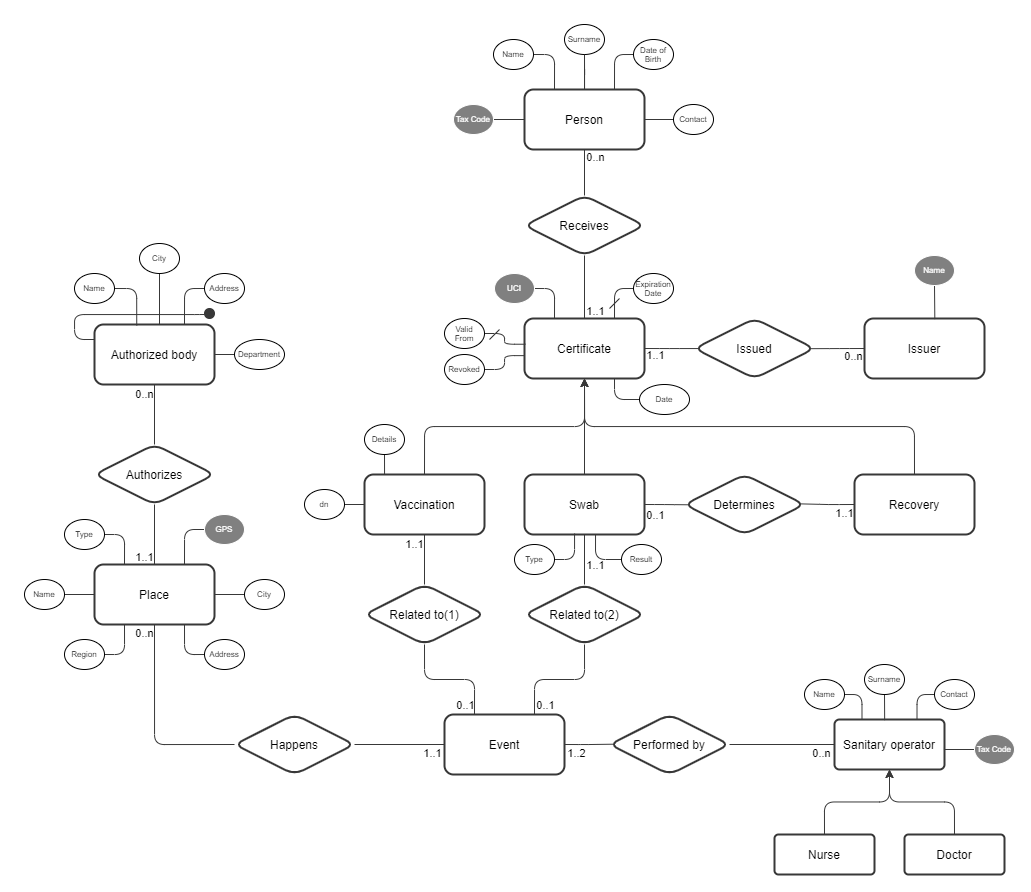
\includegraphics[scale=0.25]{er.png}
%\end{figure}
\newpage

\section{Document diagram}
The designed Document diagram is shown below. Certificate and Sanitary Operator are represented as collections of documents. Contact is a sub-document of both Certificate and Sanitary operator documents. 

The certificate document represents an unique person and it contains him/her Covid information chronology. It can have Recovery, Swab and Vaccination as sub-document and these last two have both an event details sub-document that contains all the information related to the place where the determined event happened.
\hfill\break
\\
The Recovery document has been implemented to make the recovery certificate validation easier and faster. Otherwise, doing this validation through the scan of the tests information would have been more complex due to the possibility of a person to do an unlimited amount of tests.
With this design choice the time complexity of validate a recovery certificate has been reduced.


%\begin{center}
%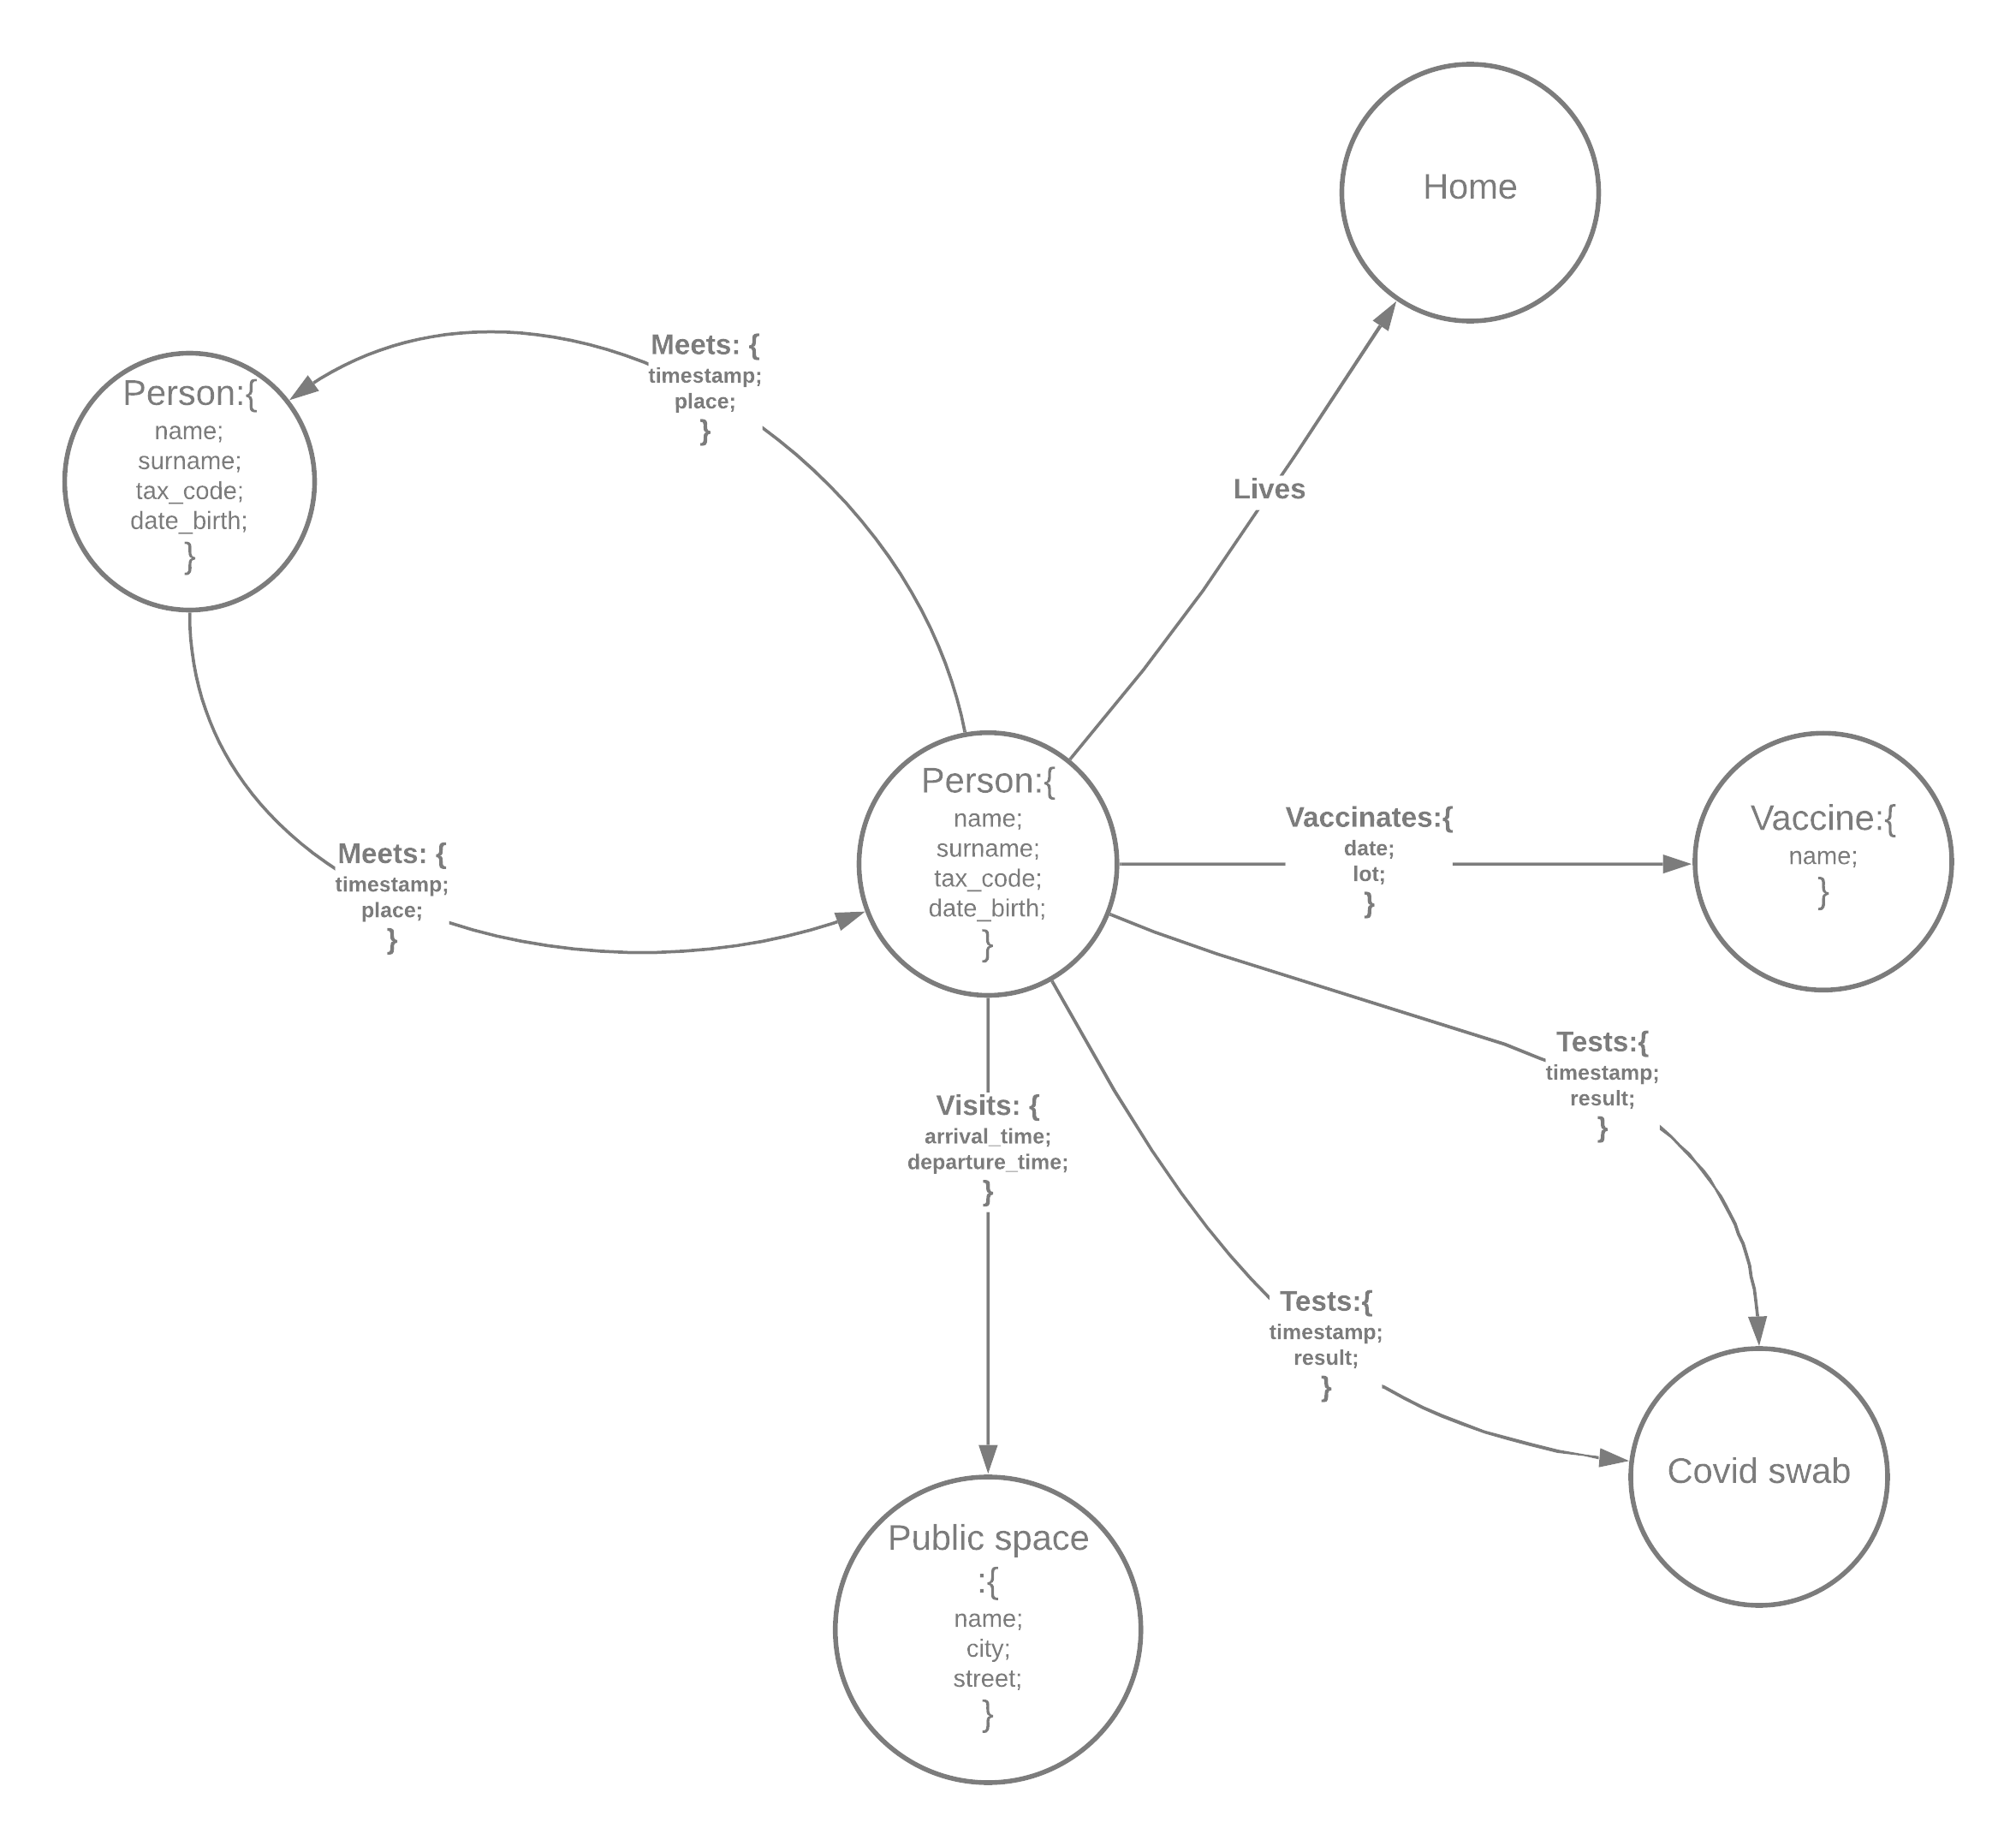
\includegraphics[scale=0.15]{Graph_diagram.png}
%\end{center}


\newpage

\section{Dataset description}
The Dataset has been built by making a script in Python, using some useful packages like: random-italian-person that automatically generates people with random attributes (this package has been modified due to our necessity); the official PyMongo driver for Python for the communication with the Database since it allows to make queries directly from Python.

\\
\hfill\break
We have also used this piece of code to generate hospitals and pharmacies data. This query has been used in overpass turbo (a web-based tool for extracting OpenStreetMap data) selecting the map area of Rome, Naples and Milan.

\begin{lstlisting}[language=cypher, label=lst:cypher-example]

CODE
\end{lstlisting}
\newpage
\section{Queries and Commands}
\subsection{Queries}
\subsubsection{Query 1}
Query description...

\begin{lstlisting}[language=cypher, label=lst:cypher-example]

CODE

\end{lstlisting}
\subsubsection{Query 2}
Query description...

\begin{lstlisting}[language=cypher, label=lst:cypher-example]

CODE

\end{lstlisting}
\subsubsection{Query 3}
Query description...

\begin{lstlisting}[language=cypher, label=lst:cypher-example]

CODE

\end{lstlisting}

\subsubsection{Query 4}
Query description...

\begin{lstlisting}[language=cypher, label=lst:cypher-example]

CODE

\end{lstlisting}
\subsubsection{Query 5}
Query description...

\begin{lstlisting}[language=cypher, label=lst:cypher-example]

CODE

\end{lstlisting}
\newpage
\subsection{Commands}
\subsubsection{Command 1}
Command description...

\begin{lstlisting}[language=cypher, label=lst:cypher-example]

CODE

\end{lstlisting}
\subsubsection{Command 2}
Command description...

\begin{lstlisting}[language=cypher, label=lst:cypher-example]

CODE

\end{lstlisting}
\subsubsection{Command 3}
Command description...

\begin{lstlisting}[language=cypher, label=lst:cypher-example]

CODE

\end{lstlisting}
\newpage
\section{Generator database}
The {\fontfamily{qcr}\selectfont"MongoDB-populator/main.py"} file is responsible of generating a random database.
In order to correctly run the generator, it is mandatory to...
%store the Neo4j password in {\fontfamily{qcr}\selectfont"neo4jDB-populator/password.txt"}, in this way the generator will be able to connect with the database.
\\This script exploits the following packages: {\fontfamily{qcr}\selectfont pandas, numpy, PyMongo and python-codicefiscale}.

\subsection{Facilities generation}
This generator will create facilities data for the following cities: Rome, Milan and Naples. For each city it will create event details representing hospitals and pharmacies available in that specific town. 
%For safety sake, the parameter that sets the number of public spaces to generate should be lower than 46.

\subsection{Certificate generation}
In order to consistently generate people certificates...

\subsection{... generation}
...


\newpage
\section{Application description}
Goal of the application {\fontfamily{qcr}\selectfont"GUI/App.py"} is to give some information about the Covid-19 Certification.
The user can use the application in order to:
\begin{itemize}
    \item Given information about a specific people, print all his valid certifications.
    \item Given a UCI, check if the related certificate is still valid, who it belongs to and its expiration date according to the actual government regulation.
\end{itemize}

%\begin{figure}[h!]
%  \centering
%  \begin{subfigure}
%    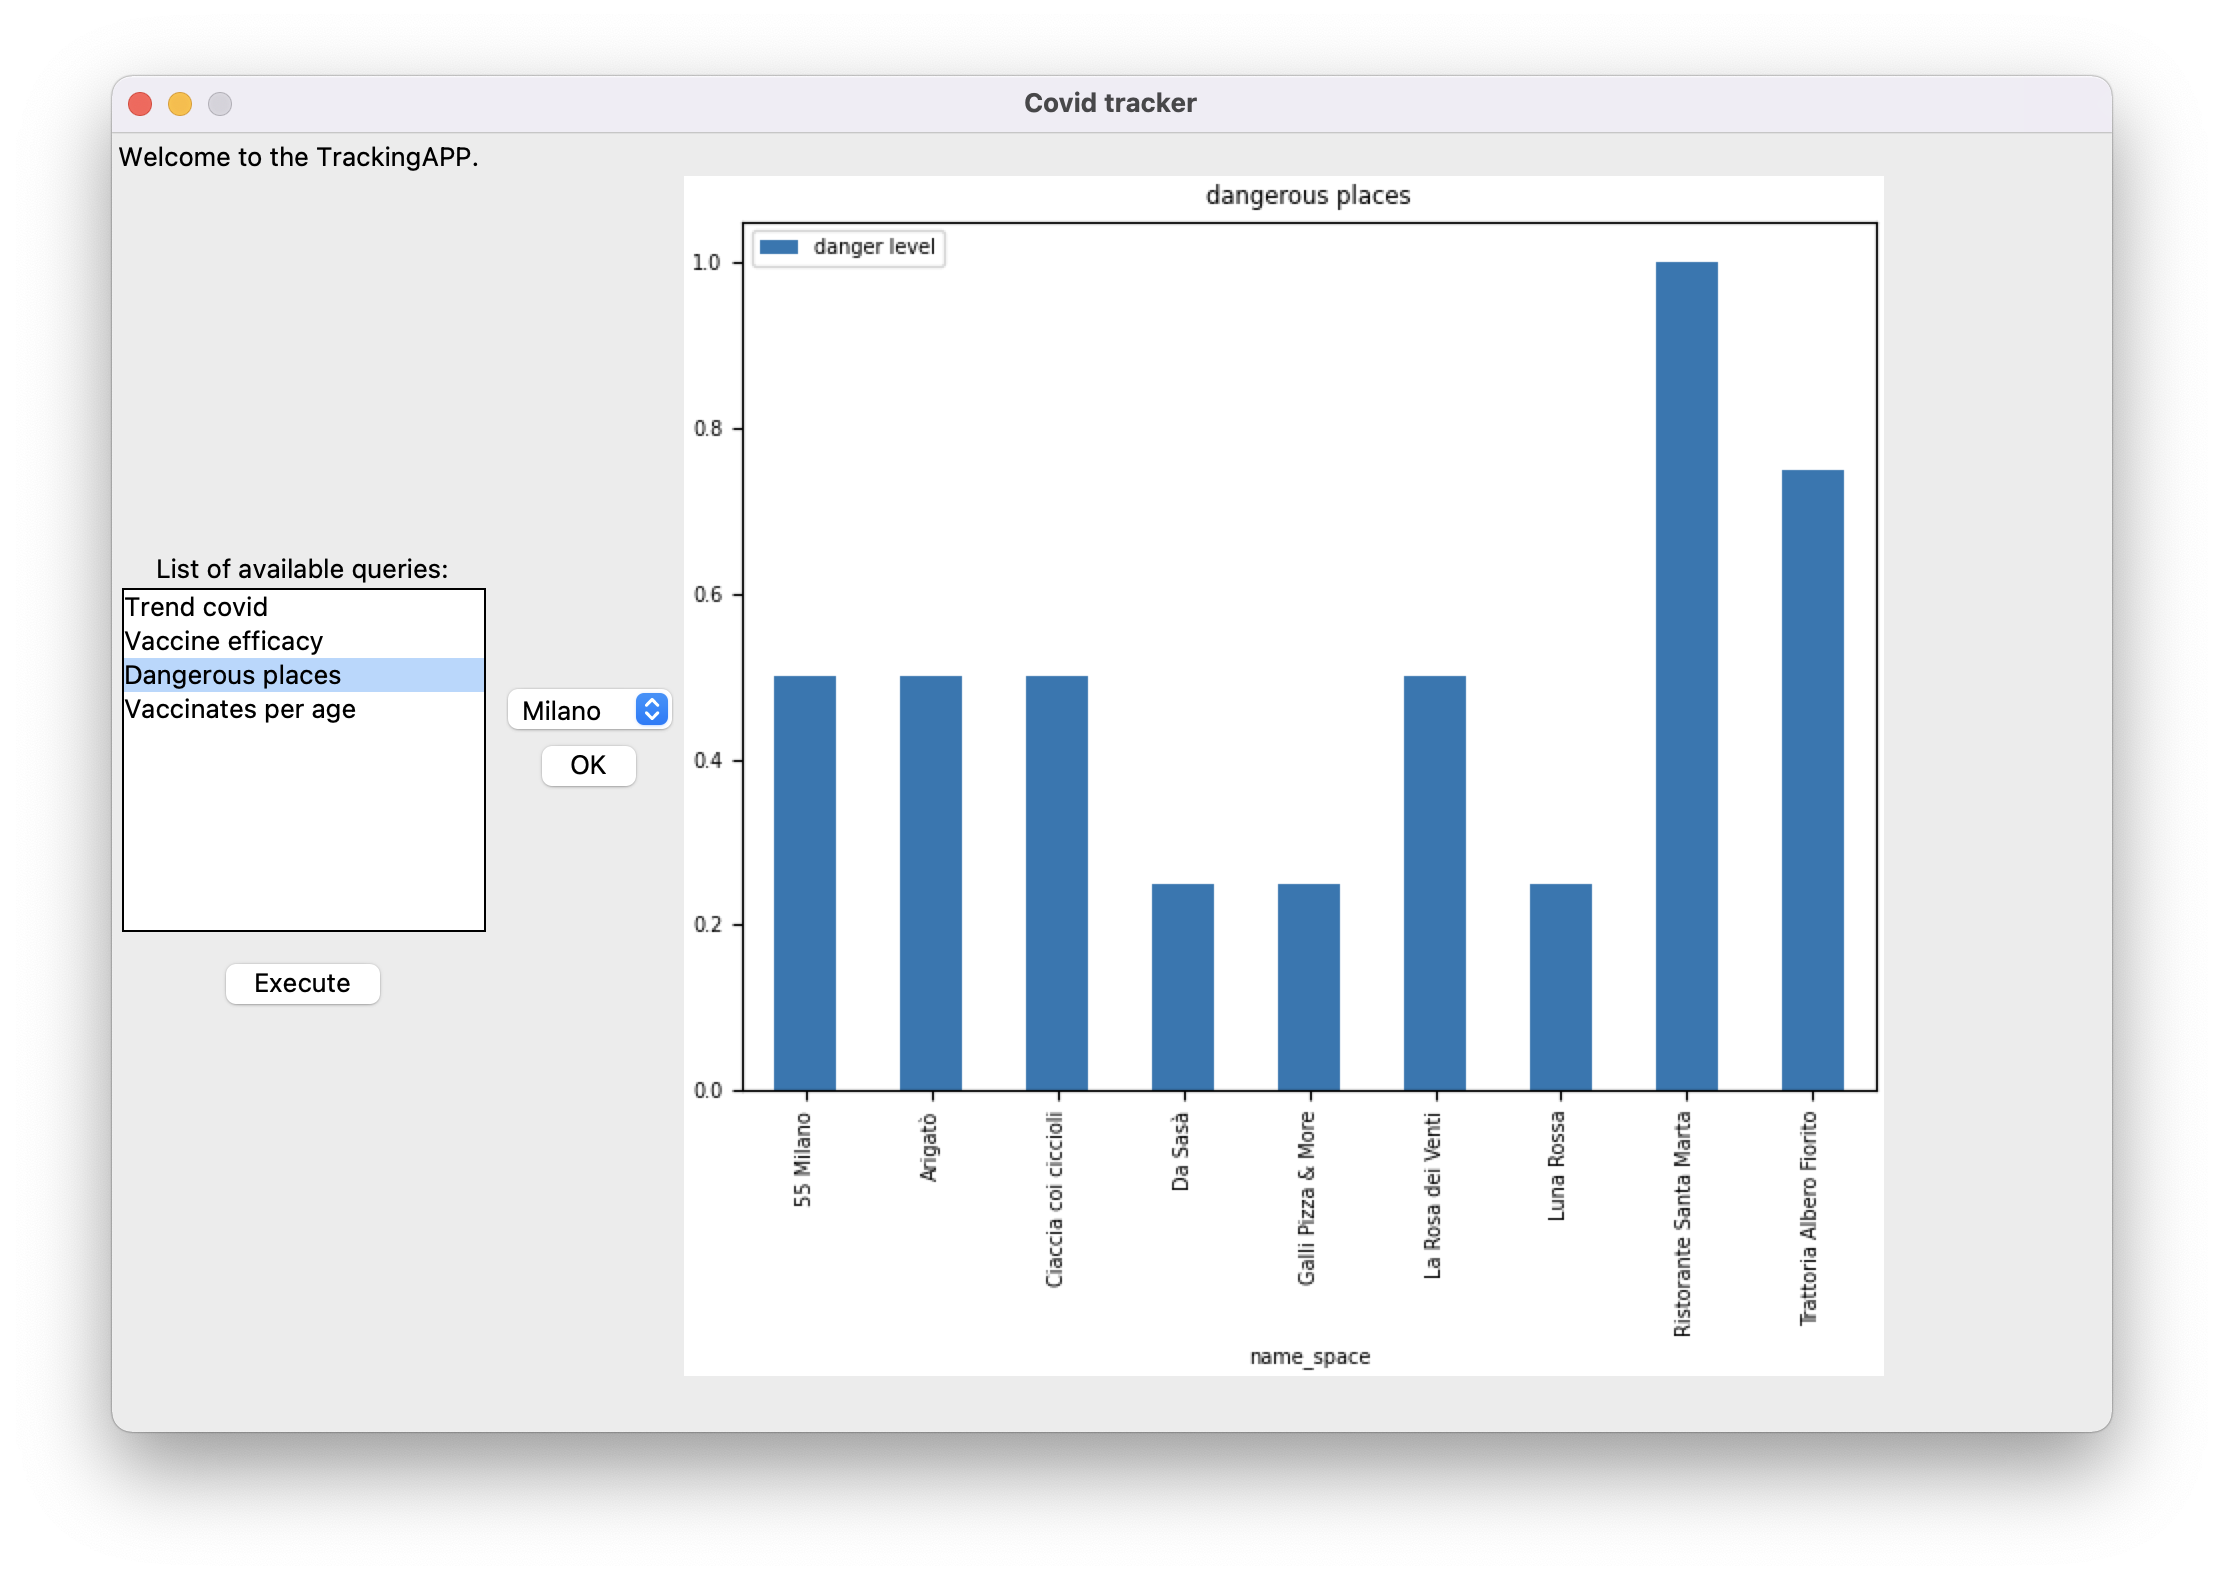
\includegraphics[scale=0.23]{danger_levels.png}
%    \caption{Application displaying danger levels in Milan.}
%  \end{subfigure}
%  \hfill \break
%  \begin{subfigure}
%    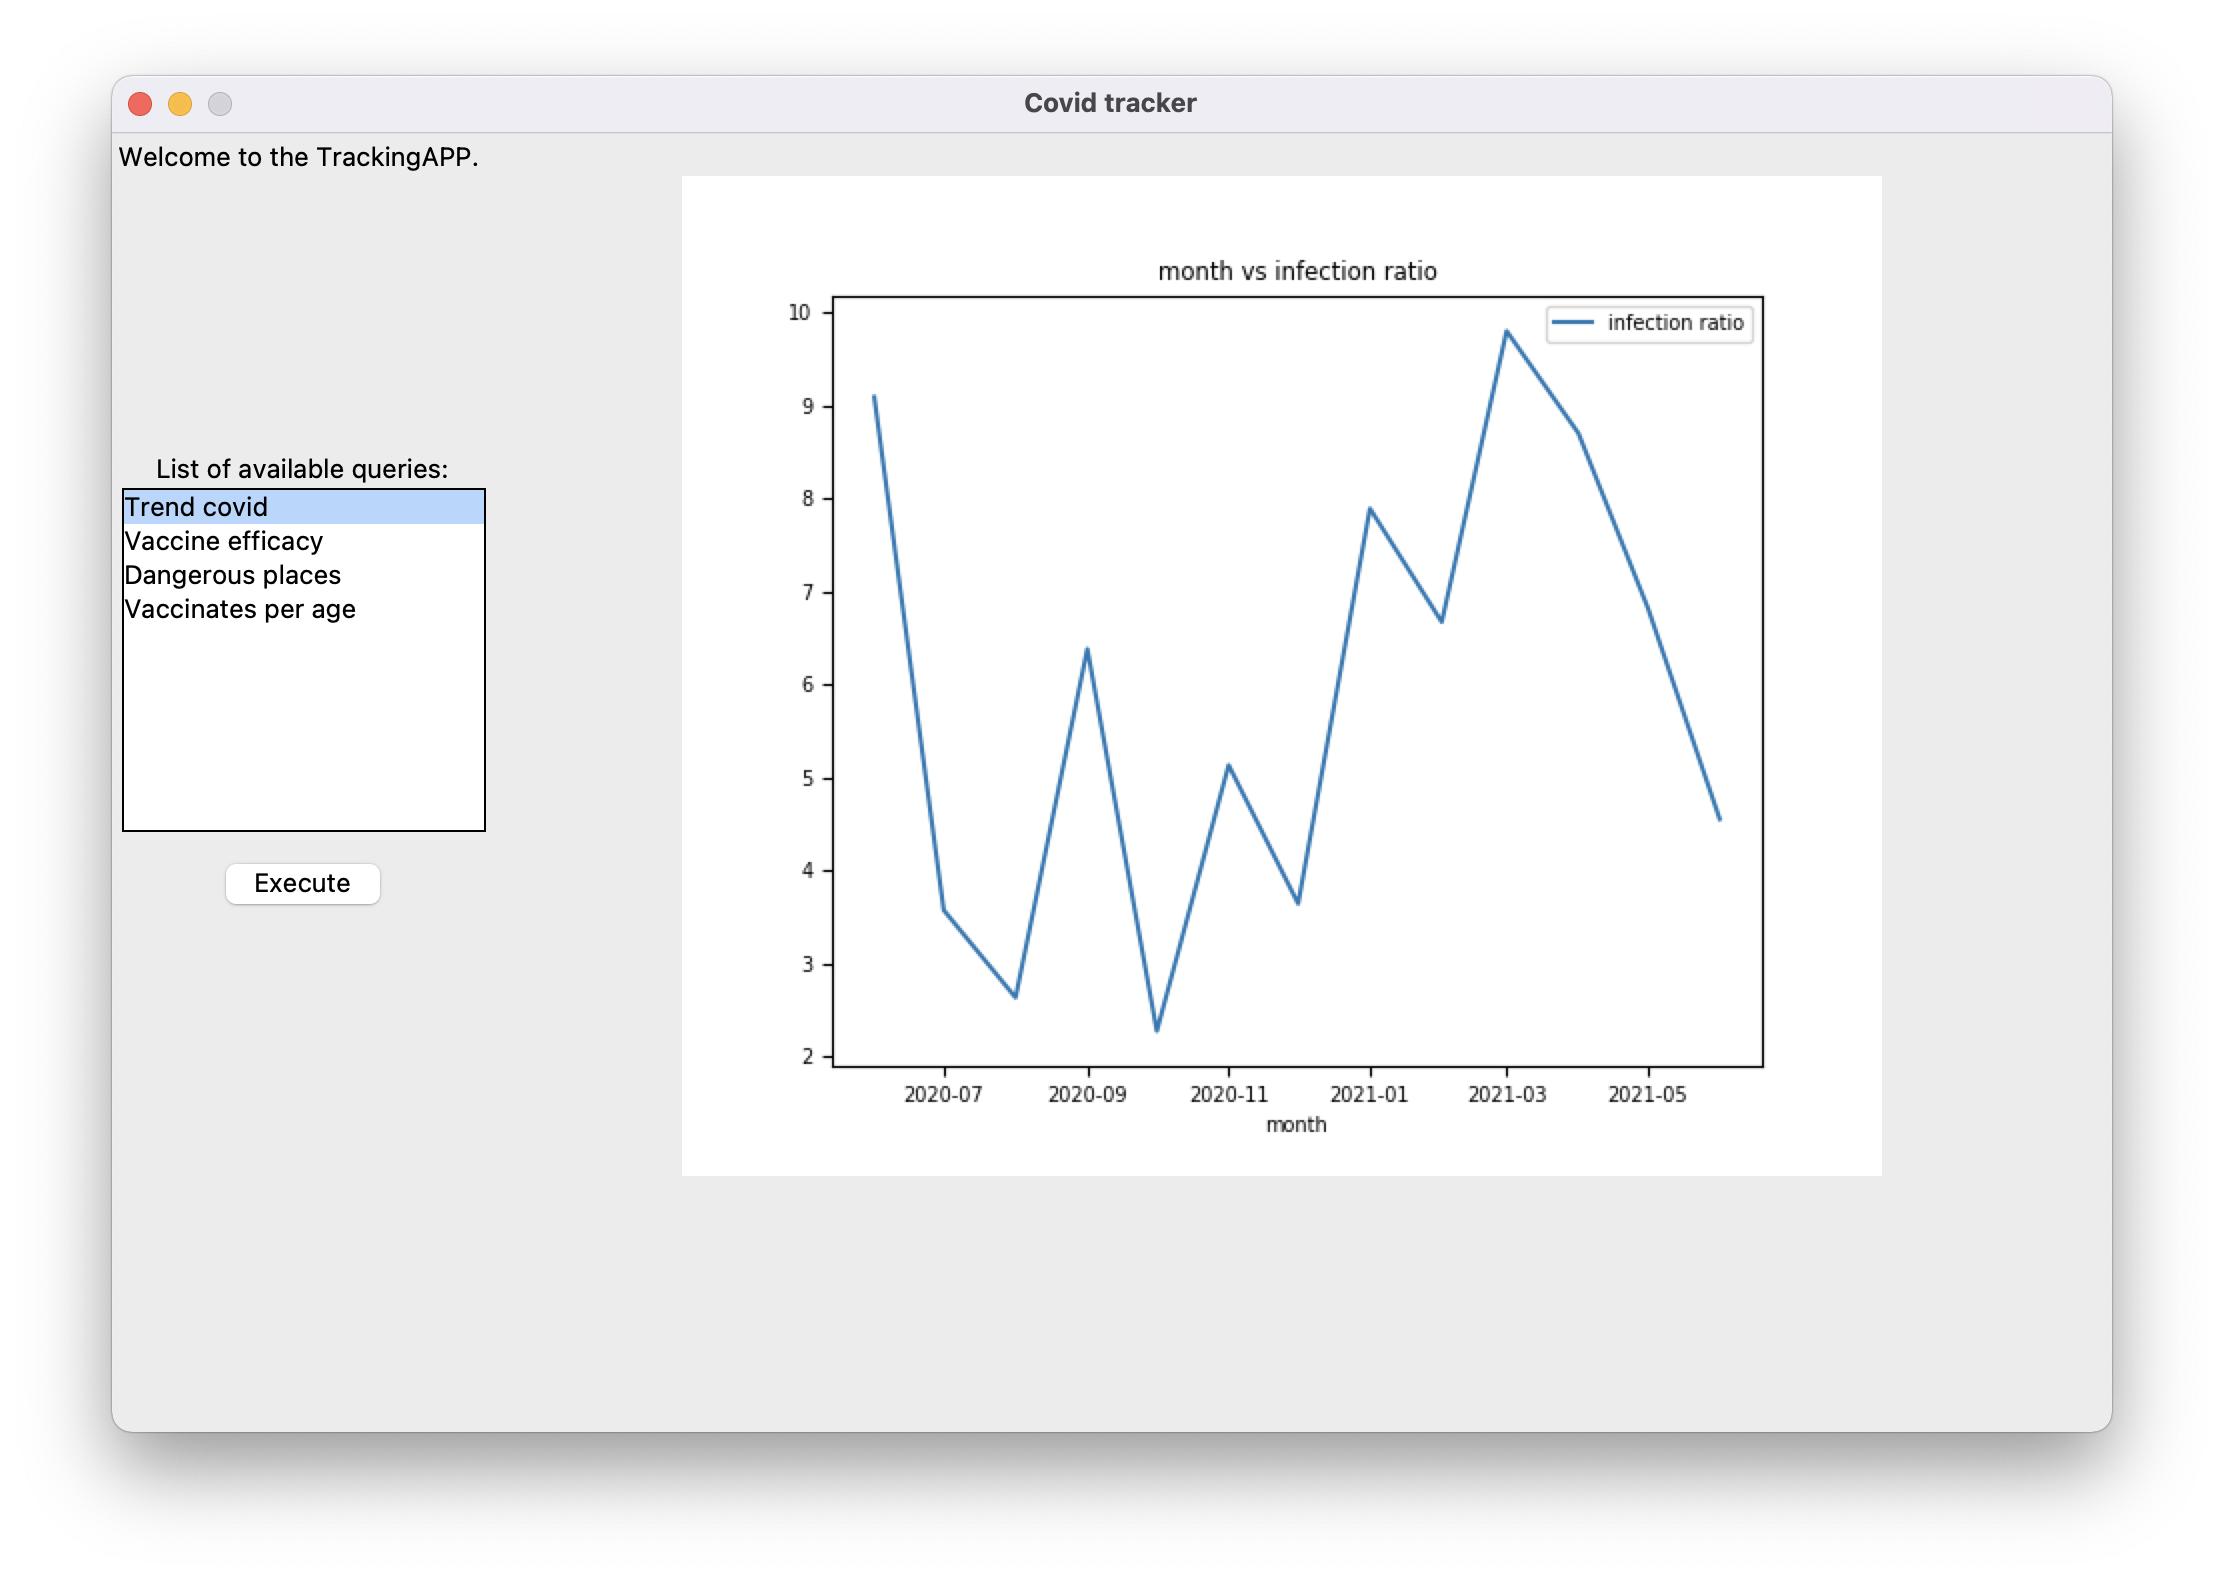
\includegraphics[scale=0.23]{trend.png}
%    \caption{Application displaying how Covid infection is spreading.}
%  \end{subfigure}
%  \label{fig:screen_from_App}
%\end{figure}

\newpage

\section{User guide}
The application is meant to work on pc or macOS. As the application has been entirely developed in Python, it is not
operative system dependent.
\\In order to correctly run the application it is mandatory to...
%store the Neo4j password in {\fontfamily{qcr}\selectfont"neo4jDB-populator/password.txt"}, in this way the application will be able to connect with the database.
\\The user must check to have installed correctly in the virtual environment the following pacakges: {\fontfamily{qcr}\selectfont tkinter, pandas, PyMongo, numpy and python-codicefiscale}.

\section{Conclusion}

Some interesting conclusions can be drawn from the development of this project: Document databases are, if well designed, easy to use and really scalable. \\

...

\section{References and Sources}
\begin{itemize}
    \item Random-italian-person package: https://pypi.org/project/random-italian-person
    \item PyMongo package: https://docs.mongodb.com/drivers/pymongo/
    \item Tkinter package: https://docs.python.org/3/library/tkinter.html
    \item Overpass turbo API: https://wiki.openstreetmap.org/wiki/Overpass\_API
\end{itemize}



\end{document}
